255. При удалении крайних клеток периметр полоски не поменяется, а при удалении соседних поменяется в сумме на 2, а должен на $50-(21+2)\cdot2=4.$ Значит, клетки необходимо удалять не крайние, не соседние и не приводящие к разваливанию полоски. Последовательно заполним полоску, написав в каждой клетке количество способов выбрать для неё вторую удаляемую клетку.
\begin{center}
\begin{figure}[ht!]
\center{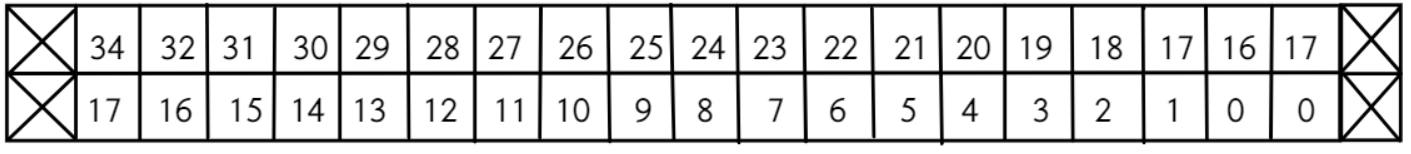
\includegraphics[scale=0.3]{gg1.png}}
\end{figure}
\end{center}
Так как крайние клетки брать нельзя, изначально для выбора остаётся $2\cdot21-4=38$ клеток. Вместе с левой верхней клеткой нельзя брать её саму и 3 её соседей, остаётся $38-4=34$ возможных клетки. Вместе со второй клеткой в верхнем ряду нельзя брать её саму и 5 соседей, остаётся $38-6=32$ возможные клетки. Далее у каждой следующей клетки будет на 1 вариант меньше (нельзя брать ранее рассмотренные клетки), пока мы не дойдём до последней клетки. Двумя её соседями являются изначально запрещённые крайние клетки, поэтому с ней можно брать $16-1+2=17$ клеток. Вместе с крайней левой клеткой нижней строки можно взять все клетки нижней строки кроме трёх с левого края и одной с правого, то есть опять $21-4=17$ клеток. Далее количество вариантов опять уменьшаться на 1, пока не дойдёт до 0. Значит, всего вариантов будет $34+32+31+30+\ldots+17+16+17+17+16+15+\ldots+2+1=1+2+\ldots+31+32+17+16+17+34=(1+32)+(2+21)+\ldots+(16+17)+84=33\cdot16+84=612.$\\
